\de{ĐỀ THI HỌC KỲ I NĂM HỌC 2022-2023}{THPT Hùng Vương}

\begin{bt}%[0T3B1-2]%[Dự án đề kiểm tra HKI NH22-23 - Nguyễn Ngọc Dũng]%[THPT Hùng Vương]
Tìm tập xác định của hàm số $y=f(x)=x^2+x+1+\sqrt{x-2022}$.
%\dapso{$\mathscr{D}=[2022;+\infty)$.}
\loigiai{
Hàm số xác định khi và chỉ khi $x-2022 \geq 0 \Leftrightarrow x \geq 2022$.\\
Vậy tập xác định của hàm số là $\mathscr{D}=[2022;+\infty)$.
}
\end{bt}

\begin{bt}%[0T3B2-1]%[Dự án đề kiểm tra HKI NH22-23 - Nguyễn Ngọc Dũng]%[THPT Hùng Vương]
Cho hàm số $y=f(x)=-x^2+2x+3$.
\begin{enumerate}
\item Lập bảng biến thiên của hàm số.
\item Dựa vào bảng biến thiên, tìm khoảng đồng biến và khoảng nghịch biến của hàm số.
\end{enumerate}
\dapso{\textbf{a)}  
\begin{tikzpicture}
\tkzTabInit[nocadre,lgt=1.2,espcl=2.5,deltacl=0.6]
{$x$/0.6,$y$/2}{$-\infty$,$1$,$+\infty$}
\tkzTabVar{-/$-\infty$,+/$4$,-/$-\infty$}
\end{tikzpicture}; \textbf{b)} Hàm số đồng biến trên $(-\infty;1)$ và nghịch biến trên $(1;+\infty)$.}
\loigiai{
\begin{enumerate}
\item \begin{itemize}
\item Đỉnh $S$ có tọa độ: $x_S=\dfrac{-b}{2a}=\dfrac{-2}{2\cdot (-1)} = 1$; $y_S=-1^2+2\cdot 1 +3 = 4$.\\
Hay $S(1;4).$
\item Vì hàm số bậc hai có $a=-1<0$ nên có bảng biến thiên như sau:
\begin{center}

\begin{tikzpicture}
\tkzTabInit[nocadre,lgt=1.2,espcl=2.5,deltacl=0.6]
{$x$/0.6,$y$/2}{$-\infty$,$1$,$+\infty$}
\tkzTabVar{-/$-\infty$,+/$4$,-/$-\infty$}
\end{tikzpicture}
\end{center}
\end{itemize}
\item Hàm số đồng biến trên $(-\infty;1)$ và nghịch biến trên $(1;+\infty)$.
\end{enumerate}
}
\end{bt}

\begin{bt}%[0T4B3-1]%[Dự án đề kiểm tra HKI NH22-23 - Nguyễn Ngọc Dũng]%[THPT Hùng Vương]
Cho tam giác $ABC$ có $AB=10$ cm, $BC=8$ cm, $AC=12$ cm.
\begin{enumerate}
\item Tính diện tích $S$ của tam giác $ABC$.
\item Tính bán kính đường tròn nội tiếp $r$ của tam giác $ABC$.
\end{enumerate}
%\dapso{\textbf{a)} $S=15\sqrt{7}$ cm$^2$; \textbf{b)} $r=\sqrt{7}$ cm.}
\loigiai{
\begin{enumerate}
\item \begin{itemize}
\item Đặt $a=BC=8$ cm, $b=AC=12$ cm, $c=AB=10$ cm.
\item Nửa chu vi tam giác $ABC$ là $p=\dfrac{a+b+c}{2} = \dfrac{8+12+10}{2}=15$ (cm).
\item Diện tích tam giác $ABC$ là 
$$S=\sqrt{p(p-a)(p-b)(p-c)} = \sqrt{15(15-8)(15-12)(15-10)}=15\sqrt{7} \text{ (cm}^2).$$
\end{itemize}
\item Ta có $r = \dfrac{S}{p} =\dfrac{15\sqrt{7}}{15}=\sqrt{7}$ (cm).
\end{enumerate}
}
\end{bt}

%Bài 4...........................
\begin{bt}%[0T5B4-1]%[Dự án đề kiểm tra HKI NH22-23-Phạm Phương]%[THPT Hùng Vương-Sở Hồ Chí Minh]
	Cho hình vuông $ABCD$ tâm $O$ và độ dài cạnh bằng $a$.
	\begin{listEX}[2]
		\item Xác định và tính góc $\left(\overrightarrow{AB},\overrightarrow{AC}\right)$.
		\item Tính tích vô hướng $\overrightarrow{AB} \cdot \overrightarrow{OC}$.
	\end{listEX}
%\dapso{\textbf{a)} $\left(\overrightarrow{AB},\overrightarrow{AC}\right)=\widehat{BAC}=45^\circ$; \textbf{b)} $\overrightarrow{AB}\cdot\overrightarrow{OC}=\dfrac{a^2}{2}$.}
\loigiai{
\immini{
\begin{enumerate}
	\item Ta có $\left(\overrightarrow{AB},\overrightarrow{AC}\right)=\widehat{BAC}$.\\
	Mà $ABCD$ là hình vuông nên $\widehat{BAC}=45^\circ$.\\
	Vậy $\left(\overrightarrow{AB},\overrightarrow{AC}\right)=45^\circ$.
	\item $\overrightarrow{AB} \cdot \overrightarrow{OC}=\left|\overrightarrow{AB}\right| \cdot \left|\overrightarrow{OC}\right|\cdot \cos \left(\overrightarrow{AB} ,\overrightarrow{OC}\right)$.
	\begin{itemize}
		\item $\left|\overrightarrow{AB}\right|=AB=a$.
		\item $\left|\overrightarrow{OC}\right|=OC=\dfrac{1}{2}AC=\dfrac{1}{2}\sqrt{a^2+a^2}=\dfrac{a\sqrt{2}}{2}$.
		\item $\left(\overrightarrow{AB} ,\overrightarrow{OC}\right)=\left(\overrightarrow{AB} ,\overrightarrow{AO}\right)=\widehat{BAO}=45^{\circ}$. 
	\end{itemize}
	Vậy $\overrightarrow{AB} \cdot \overrightarrow{OC}= a\cdot \dfrac{a\sqrt{2}}{2}\cdot \cos 45^{\circ}=\dfrac{a^2}{2}$.
\end{enumerate}
}{
\begin{tikzpicture}[scale=1,>=stealth, font=\footnotesize, line join=round, line cap=round]
	\foreach \i/\j/\k in{0/0/A,0/-3/B,3/-3/C,3/0/D}
	\coordinate (\k) at(\i,\j);
	\draw (A)--(B)--(C)--(D)--cycle
	(A)--(C)(B)--(D);
	\coordinate (O) at ($(A)!0.5!(C)$);
	\foreach \p/\r in {A/135,B/-135,C/45,D/45,O/-90}
	\fill (\p) circle (1pt) node[shift={(\r:3mm)}]{$\p$};
	\node at ($(A)!0.5!(B)$)[left]{$a$};
	\draw (A)pic[draw=black, angle eccentricity=1.6, angle radius=0.3cm,rotate=-67.5]{angle=B--A--C};
	\node at (A)[shift={(-67.5:6mm)},rotate=-67.5]{$45^\circ$};
\end{tikzpicture}
}
}
\end{bt}
%Bài 5...........................
\begin{bt}%[0T6B3-1]%[0T6B3-2]%[0T6B3-3]%[Dự án đề kiểm tra HKI NH22-23-Phạm Phương]%[THPT Hùng Vương-Sở Hồ Chí Minh]
	Bảng sau đây cho biết sức chứa dành cho khán giả của các sân vận động được sử dụng trong nhiều sự kiện thể thao tại Việt Nam \textit{(số liệu gần đúng)}.
	\begin{center}
		\begin{tabular}{|c|c|c|c|c|c|c|c|c|c|}
			\hline
			$\begin{array}{*{20}{c}}
				\text{Sân}\\
				\text{vận}\\
				\text{động}
			\end{array}$ 
			& $\begin{array}{*{20}{c}}
				\text{Thống}\\
				\text{Nhất}
			\end{array}$ 
			& Tự Do
			& $\begin{array}{*{20}{c}}
				\text{Hòa}\\
				\text{Xuân}
			\end{array}$ 
			& $\begin{array}{*{20}{c}}
				\text{Hàng}\\
				\text{Đẫy}
			\end{array}$ 
			& $\begin{array}{*{20}{c}}
				\text{Đồng}\\
				\text{Nai}
			\end{array}$ 
			& $\begin{array}{*{20}{c}}
				\text{Lạch}\\
				\text{Tray}
			\end{array}$ 
			& $\begin{array}{*{20}{c}}
				\text{Thiên}\\
				\text{Trường}
			\end{array}$
			& $\begin{array}{*{20}{c}}
				\text{Cần}\\
				\text{Thơ}
			\end{array}$
			& $\begin{array}{*{20}{c}}
				\text{Mỹ}\\
				\text{Đình}
			\end{array}$\\
			\hline
			$\begin{array}{*{20}{c}}
				\text{Sức}\\
				\text{chứa}
			\end{array}$ & $15\,000$ & $16\,000$ & $20\,500$ & $22\,500$ & $30\,000$ & $30\,000$ & $30\,000$ & $30\,000$ & $40\,190$\\
			\hline
		\end{tabular}
	\end{center}
	\begin{flushright}
		\textit{(Nguồn: Wikipedia)}
	\end{flushright}
Hãy tìm số trung bình, tứ phân vị và mốt của mẫu số liệu trên.
%\dapso{$\overline{x}=\dfrac{234190}{9}$; $M_0=30\,000$; $Q_1=18\,250$; $Q_2=30\,000$; $Q_3=30\,000$.}
	\loigiai{
\begin{itemize}
	\item Số trung bình là $$\overline{x}=\dfrac{1}{9}\left(15\,000+16\,000+20\,500+22\,500+4\cdot 30\,000+40\,190\right)\approx 26\,021.$$
	\item Tứ phân vị của dãy số liệu là
	\begin{itemize}
		\item $Q_1=\dfrac{16\,000+20\,500}{2}=18\,250$.
		\item $Q_2=30\,000$.
		\item $Q_3=\dfrac{30\,000+30\,000}{2}=30\,000$.
	\end{itemize}	
	\item Giá trị $30\,000$ xuất hiện nhiều nhất (4 lần) nên mốt là $M_o=30\,000$.
\end{itemize}	
}
\end{bt}
%Bài 6...........................
\begin{bt}%[0T4B3-1]%[Dự án đề kiểm tra HKI NH22-23-Phạm Phương]%[THPT Hùng Vương-Sở Hồ Chí Minh]
	\immini{Một ô tô muốn đi từ $A$ đến $C$, nhưng giữa $A$ và $C$ là một ngọn núi cao nên ô tô phải đi đường tránh thành hai đoạn từ $A$ đến $B$ rồi từ $B$ đến $C$, các đoạn đường tạo thành tam giác $ABC$ có độ dài $AB=15\,\mathrm{km}$, $BC=20\,\mathrm{km}$ và $\widehat{ABC}=60^\circ$. Để rút ngắn khoảng cách và tránh sạt lở núi, người ta dự định làm đường hầm xuyên núi nối thẳng từ $A$ đến $C$. Hỏi quãng đường từ $A$ đến $C$ dài bao nhiêu? \textit{(Kết quả làm tròn đến chữ số thập phân thứ hai)}.}
	{\definecolor{tumbleweed}{rgb}{0.87, 0.67, 0.53}%màu cát	
		\definecolor{battleshipgrey}{rgb}{0.52, 0.52, 0.51}
		\definecolor{darkgray}{rgb}{0.66, 0.66, 0.66}
		\definecolor{dimgray}{rgb}{0.41, 0.41, 0.41}
		\definecolor{forestgreen(web)}{rgb}{0.13, 0.55, 0.13}
		\definecolor{darkpastelgreen}{rgb}{0.01, 0.75, 0.24}
		\definecolor{cadmiumgreen}{rgb}{0.0, 0.42, 0.24}
		\begin{tikzpicture}[line join=round, line cap=round,scale=1,transform shape]
			%\fill[tumbleweed] (-6,-2) rectangle (6,-.4);
			\tikzset{nui/.pic={
					\def\N{ 
						(-4.2,-.8)
						..controls +(42:1) and +(-140:1) ..  (-2,.55)
						..controls +(45:1) and +(-140:1) ..  (-.6,1.65)%đỉnh núi
						..controls +(-25:.2) and +(140:.2) ..  (-.15,1.25)
						..controls +(-25:.2) and +(140:.2) ..  (.4,.95)
						..controls +(-25:.5) and +(140:.5) ..  (2,.2)
						..controls +(-45:.5) and +(140:.5) ..  (4.5,-.85)%chân núi phải
						..controls +(165:.8) and +(5:.5) ..  (1,-.8)
						..controls +(-175:.8) and +(5:1) ..  (-2,-.8)
						..controls +(-175:.8) and +(-5:1) ..  (-4.2,-.8);}
					\draw \N;
					\fill[darkgray] \N;
					\def\T{ %Bóng núi phải
						(-.6,1.65)%đỉnh núi
						..controls +(-25:.2) and +(140:.2) ..  (-.15,1.25)
						..controls +(-25:.2) and +(140:.2) ..  (.4,.95)
						..controls +(-25:.5) and +(140:.5) ..  (2,.2)
						..controls +(-45:.5) and +(140:.5) ..  (4.5,-.8)%chân núi phải
						..controls +(165:.8) and +(-30:.3) ..  (3,-.7)
						..controls +(165:.8) and +(-25:.5) ..  (1.5,-.2)
						..controls +(165:.8) and +(-25:.5) ..  (.7,.2)
						..controls +(165:.8) and +(-55:.5) ..  (-.6,1.65);}
					\draw \T;
					\fill[dimgray] \T;}}	
			\path 
			%(2.2,-.2)pic[scale=.8]{nui}
			%(-2,0)pic[scale=.6]{nui}
			(1,0.4)pic[scale=0.5]{nui};
			\coordinate [label=above:$A$] (A) at (-2,0);
			\coordinate [label=above:$C$] (C) at (5,0);
			\coordinate [label=below:$B$] (B) at (-3.5,-3);
			\foreach \point in {A,B,C} \fill[black] (\point) circle (2pt);
			\draw[line width=1pt] (A)--(B)--(C)--(A);
	\end{tikzpicture}}
	%\dapso{$AC=5\sqrt{13}\,\mathrm{km}\approx 18{,}03\,\mathrm{km}$.}
	\loigiai{
Áp dụng định lý cô-sin cho tam giác $ABC$ ta có
\allowdisplaybreaks\begin{eqnarray*}
	& &AC^2=AB^2+BC^2-2\cdot AB\cdot BC\cdot \cos B \\
	&\Leftrightarrow & AC^2=15^2+20^2-2\cdot 15\cdot 20\cdot \cos 60^\circ =325\\
	&\Rightarrow & AC=\sqrt{325}=5\sqrt{13}\approx 18{,}03 \mathrm{\,km}.
\end{eqnarray*}
}
\end{bt}
%Bài 7...........................
\begin{bt}%[0T3K2-5]%[Dự án đề kiểm tra HKI NH22-23-Phạm Phương]%[THPT Hùng Vương-Sở Hồ Chí Minh]
\immini{
Khi một quả bóng được đá lên nó sẽ đạt được độ cao nào đó rồi rơi xuống đất. Biết quỹ đạo của quả bóng là một đường parabol trong mặt phẳng toạ độ $Oth$ có phương trình $h(t)=at^2+bt+c$ $(a<0)$, trong đó $t$ là thời gian (tính bằng giây) kể từ khi quả bóng được đá lên và $h$ là độ cao (tính bằng mét) của quả bóng. Giả thiết rằng quả bóng được đá lên từ độ cao $1$ m và sau $1$ giây thì nó đạt được độ cao $6{,}5$ m, sau $4$ giây nó đạt độ cao $5$ m. Hãy xác định độ cao cao nhất mà quả bóng đã đạt được?
}{
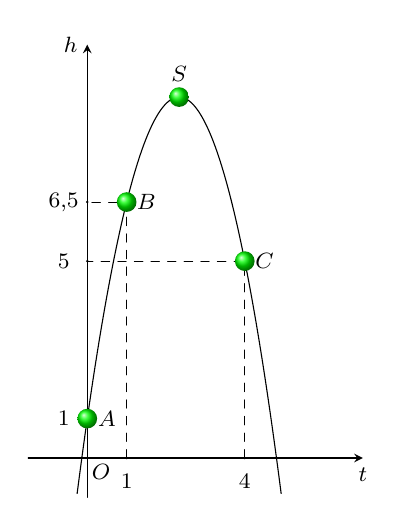
\begin{tikzpicture}[scale=0.5,>=stealth, font=\footnotesize, line join=round, line cap=round]
	\def\a{-1.5} \def\b{7} \def\c{1} % Hệ số
	\def\xmin{-1.5} \def\xmax{7}
	\def\ymin{-1} \def\ymax{10.5}
	%\draw[color=gray!50,dashed] (\xmin,\ymin) grid (\xmax,\ymax);
	\draw[->] (\xmin,0)--(\xmax,0) node [below]{$t$};
	\draw[->] (0,\ymin)--(0,\ymax) node [left]{$h$};
	\fill (0,0) circle (1pt) node[shift={(-45:2.5mm)}]{$O$};
	\node at (0,1) [shift={(0:2.5mm)}]{$A$};
	\node at (1,6.5) [shift={(0:2.5mm)}]{$B$};
	\node at (4,5) [shift={(0:2.5mm)}]{$C$};
	\node at (7/3,55/6) [shift={(90:3mm)}]{$S$};
	\clip (\xmin+0.1,\ymin+0.1) rectangle (\xmax-0.5,\ymax-0.1);
	\draw[smooth,samples=300,domain=\xmin:\xmax] plot(\x,{\a*(\x)^2+\b*(\x)+\c});
	\draw[dashed] (1,0)|-(0,6.5) (4,0)|-(0,5);
	\foreach \s/\t in {1/-90,4/-90}%Trục Ox
	\fill (\s,0) circle (1pt) node[shift={(\t:3mm)}]{$\s$};
	\foreach \p/\r in {1/180,5/180}%Trục Oy
	\fill (0,\p) circle (1pt) node[shift={(\r:3mm)}]{$\p$};
	\fill (0,6.5) circle (1pt) node[shift={(180:3mm)}]{$6{,}5$};
	\shade[ball color=green] (0,1) circle (.25cm);
	\shade[ball color=green] (1,6.5) circle (.25cm);
	\shade[ball color=green] (7/3,55/6) circle (.25cm);
	\shade[ball color=green] (4,5) circle (.25cm);
\end{tikzpicture}
}
	%\dapso{$\dfrac{55}{6}\,\mathrm{m}\approx 9{,}17\,\mathrm{m}$.}
	\loigiai{
Xét hàm số $h(t)=at^2+bt+c$. Theo giả thiết đề bài ta có
$$\heva{&h(0)=1\\&h(1)=6{,}5\\&h(4)=5}\Leftrightarrow\heva{&c=1\\&a+b+c=6{,}5\\&16a+4b+c=5} \Leftrightarrow \heva{&a=-\dfrac{3}{2}\\&b=7\\&c=1.}$$
Khi đó parabol có phương trình là $h(t)=-\dfrac{3}{2}t^2+7t+1$.
Đỉnh $S$ của parabol có toạ độ là
\begin{itemize}
	\item $x_S=-\dfrac{b}{2a}=\dfrac{-7}{2\cdot \left(-\tfrac{3}{2}\right)}=\dfrac{7}{3}$.
	\item $y_S=y\left(\dfrac{7}{3}\right)=-\dfrac{3}{2}\left(\dfrac{7}{3}\right)^2+7\left(\dfrac{7}{3}\right)+1=\dfrac{55}{6}\approx 9{,}17$.
\end{itemize}
Vậy  độ cao cao nhất mà quả bóng đã đạt được là $9{,}17$ m.
}
\end{bt}


